%==========================================================================
%  Community Security Alert System (CSAS)
%  Workshop No. 3 — Robust System Design and Project Management
%  REVISED VERSION
%
%  Universidad Distrital Francisco José de Caldas
%  Computer Engineering — Semester 2026-I
%  Instructor: Eng. Carlos Andrés Sierra, M.Sc.
%
%  Authors:
%    Felipe José Garzón Herrera        20251020132
%    Juan Esteban Quintero Gordillo    20251020137
%    Henry Samuel Garrido Medina       20251020125
%    Gabriel Mateo Cusba Marín         20251020128
%
%  REVISION NOTES
%  This version addresses all professor feedback from the first submission:
%  (1)  Re-centred on complete system (people + processes + technology),
%       not only software components.
%  (2)  Explicit section-level traceability from every W3 decision
%       to a specific W1 observation or W2 design choice.
%  (3)  Agile planning replaced the sequential Gantt: product backlog,
%       four sprints with goals, and a hybrid milestone frame.
%  (4)  Quality attributes traced to stakeholder needs, not just standards.
%  (5)  Risk register expanded to include organisational and behavioural
%       risks; each risk cites the W1/W2 finding that first revealed it.
%  (6)  Writing rewritten for coherence, transitions, and precise
%       technical language throughout.
%==========================================================================

\documentclass[12pt,a4paper]{article}

%------ Packages -----------------------------------------------------------
\usepackage[margin=2.5cm,top=2.8cm,bottom=2.8cm]{geometry}
\usepackage[utf8]{inputenc}
\usepackage[T1]{fontenc}
\usepackage{lmodern}
\usepackage{microtype}
\usepackage{graphicx}
\usepackage{booktabs}
\usepackage{array}
\usepackage{tabularx}
\usepackage{multirow}
\usepackage{longtable}
\usepackage{enumitem}
\usepackage{amsmath}
\usepackage{xcolor}
\usepackage{fancyhdr}
\usepackage{titlesec}
\usepackage{caption}
\usepackage[hidelinks]{hyperref}

\usepackage{tikz}
\usetikzlibrary{shapes.geometric,arrows.meta,positioning,calc,fit,matrix}

%------ Colours ------------------------------------------------------------
\definecolor{udblue}{HTML}{003087}
\definecolor{udgold}{HTML}{C8962E}
\definecolor{soft}{HTML}{F5F5F5}
\definecolor{crit}{HTML}{B53737}
\definecolor{high}{HTML}{C07020}
\definecolor{med}{HTML}{C8962E}
\definecolor{low}{HTML}{1B7F3A}

%------ Page style ---------------------------------------------------------
\pagestyle{fancy}\fancyhf{}
\fancyhead[L]{\small\color{udblue}CSAS — Workshop No.\ 3 (Revised) — Robust Design \& Project Management}
\fancyhead[R]{\small\color{udblue}Semester 2026-I}
\fancyfoot[C]{\small\thepage}
\renewcommand{\headrulewidth}{0.4pt}

%------ Section formatting -------------------------------------------------
\titleformat{\section}[block]
  {\large\bfseries\color{udblue}}{\thesection.}{0.5em}{}[\vspace{-4pt}\rule{\linewidth}{0.4pt}]
\titleformat{\subsection}[runin]
  {\normalsize\bfseries}{\thesubsection.}{0.5em}{}[\ ---\ ]
\titleformat{\subsubsection}[runin]
  {\normalsize\itshape}{\thesubsubsection.}{0.5em}{}[\ ---\ ]

%------ Misc ---------------------------------------------------------------
\renewcommand{\arraystretch}{1.25}
\setlist[enumerate]{itemsep=2pt,parsep=0pt}
\setlist[itemize]{itemsep=2pt,parsep=0pt}
\captionsetup{font=small,labelfont=bf}

%==========================================================================
\begin{document}

%------ Title page ---------------------------------------------------------
\begin{titlepage}
\centering\vspace*{1.5cm}
{\color{udblue}\rule{\linewidth}{1.5pt}}\vspace{4pt}
{\color{udgold}\rule{\linewidth}{4pt}}\vspace{16pt}

{\LARGE\bfseries\color{udblue}Community Security Alert System (CSAS)}\\\vspace{6pt}
{\large\bfseries Robust System Design and Project Management}\\\vspace{4pt}
{\large Workshop No.\ 3 --- Revised Submission}\\\vspace{16pt}

{\color{udgold}\rule{\linewidth}{4pt}}\vspace{4pt}
{\color{udblue}\rule{\linewidth}{1.5pt}}\vspace{24pt}

\begin{tabular}{ll}
\textbf{Authors} & Felipe José Garzón Herrera \hfill 20251020132\\
& Juan Esteban Quintero Gordillo \hfill 20251020137\\
& Henry Samuel Garrido Medina \hfill 20251020125\\
& Gabriel Mateo Cusba Marín \hfill 20251020128\\[8pt]
\textbf{Course} & Systems Analysis and Design\\
\textbf{Instructor} & Eng.\ Carlos Andrés Sierra, M.Sc.\\
\textbf{Program} & Computer Engineering\\
\textbf{Institution} & Universidad Distrital Francisco José de Caldas\\
\textbf{Semester} & 2026-I\\
\end{tabular}

\vfill
{\small\color{gray}
Document type: Systems Engineering Technical Report.
This document is the third stage of the CSAS project.
It builds on the systems analysis of Workshop~1 and the
system design of Workshop~2 by adding robustness, quality,
risk, and project management layers to the complete
socio-technical system — people, processes, and technology.}
\end{titlepage}

\tableofcontents\newpage

%==========================================================================
\section{Introduction and Workshop Scope}

This document constitutes the third and final stage of the CSAS
project cycle. Workshops~1 and~2 established what the campus safety
system looks like today and what changes it needs; this workshop
answers a different question: \emph{how do we make the proposed
intervention robust, auditable, and manageable as a real project?}

To answer that question rigorously, we found it necessary to hold
onto the systems engineering principle that guided Workshop~2: the
unit of analysis is the \emph{complete system} --- people, processes,
and technology together --- not the software platform alone. This
distinction matters for robustness. A system can fail at the
organisational layer (security staff do not adopt the new workflow)
or at the environmental layer (rain degrades GPS signal during the
exact hours when most incidents occur) just as easily as it can fail
at the software layer (a service crashes under load). Robustness that
covers only software failures is not robustness; it is partial
hardening.

The three additions that Workshop~3 makes to the existing design are:
(i) a \emph{system-level robustness specification} that extends the
Workshop~2 architecture into its human and organisational dimensions;
(ii) a \emph{quality and risk framework} grounded in the specific
operational findings of Workshop~1, not in generic standards;
and (iii) a \emph{project plan} built around genuine agile
iteration cycles, with a product backlog traceable to user needs
rather than a sequential schedule dressed up as agile.

Table~\ref{tab:w3scope} positions Workshop~3 within the three-workshop
progression.

\begin{table}[h]
\caption{Three-workshop progression and Workshop~3 scope}
\label{tab:w3scope}
\centering
\begin{tabularx}{\textwidth}{lXXX}
\toprule
\textbf{Dimension} & \textbf{Workshop 1} & \textbf{Workshop 2} & \textbf{Workshop 3 (this document)} \\
\midrule
Primary question & What is wrong with the system? & How should the system be designed? & How do we build and manage it robustly? \\
Focus & Empirical system characterisation & Architecture and operational design & Robustness, quality, risk, and project management \\
Quality attributes & Identified as gaps & Specified as requirements & Measured, bounded, and traced to stakeholders \\
Risks & Surfaced (assumptions unvalidated) & Partially addressed in DDRs & Registered, scored, and assigned to sprints \\
Project management & None & Outline phases & Agile sprint plan with backlog and goals \\
Standards & Cited as motivation & Referenced in DDRs & Mapped to components and acceptance criteria \\
\bottomrule
\end{tabularx}
\end{table}

%==========================================================================
\section{System-Level Robustness}
\label{sec:robustness}

\subsection{Why system-level robustness differs from software robustness.}
When we reviewed our Workshop~2 design through the lens of this
workshop, we noticed that most of our robustness mechanisms addressed
software-layer failures: service crashes, network partitions,
database unavailability. These are important, but they represent
only one dimension of the risk space. Our Workshop~1 fieldwork
identified two failure modes that sit \emph{outside} the software
layer and that have at least as much potential to undermine the
system's goals.

The first is \emph{organisational failure}: if the campus security
team does not change its operational workflow to incorporate CSAS
alert data, the system can broadcast every verified incident
perfectly and still produce no improvement in response time.
The second is \emph{environmental failure}: both suspicious events
we observed during fieldwork coincided with rainy nights when foot
traffic was low and GPS signal quality was degraded. A system that
relies entirely on mobile GPS and push notifications is structurally
vulnerable during precisely the conditions when campus risk is
highest.

Accordingly, this section specifies robustness across three
layers: technical, organisational, and environmental.

\subsection{Technical robustness.}
The software architecture inherited from Workshop~2 provides the
technical robustness baseline. Table~\ref{tab:techrobust} summarises
the mechanisms, the quality attribute each protects, and the
Workshop~1 or Workshop~2 finding that made each mechanism necessary.

\begin{table}[h]
\caption{Technical robustness mechanisms with traceability}
\label{tab:techrobust}
\centering
\begin{tabularx}{\textwidth}{p{3.2cm}Xp{2.8cm}p{3.5cm}}
\toprule
\textbf{Mechanism} & \textbf{What it protects} & \textbf{Quality attr.} & \textbf{W1/W2 finding that motivated it} \\
\midrule
Kubernetes auto-scaling on Verification Engine and Dispatcher pods & Alert latency under surge; NFR-01 ($<$30\,s) & Scalability & W1: user participation is non-linear — small user-count increase produces disproportionate report spike \\
RabbitMQ priority queues (CRITICAL / HIGH / STANDARD lanes) & CRITICAL alerts bypass STANDARD backlog & Reliability & W2 DDR-02: multiplicative priority model requires separate processing paths \\
PostgreSQL primary-standby replication + WAL & Zero incident data loss on DB failure & Reliability & W1: only 41\% of events are currently recorded; every verified record is irreplaceable \\
Multi-AZ API gateway with automatic failover & Submission availability during AZ outage & Availability & NFR-03: guaranteed uptime during 18:00--22:00, the highest-risk window identified in W1 \\
SMS fallback activated after 10-second push timeout & Alert delivery when push channel fails & Reliability & W1 benchmarking: existing platforms fail when users lack smartphone or connectivity \\
Offline report queue in the mobile app & Report submission in connectivity dead zones & Availability & W1: signal coverage across campus zones was not assessed; dead zones are a known risk \\
TLS~1.3 in transit + AES-256 at rest + role-based access control & Personal data protection & Security & Ley 1581/2012 compliance; W1 data collection included personal identifiers \\
\bottomrule
\end{tabularx}
\end{table}

\subsection{Organisational robustness.}
Technical mechanisms protect the platform; organisational mechanisms
protect the \emph{system's ability to achieve its goals}. The
distinction matters because the CSAS goals --- reduce response time
from 11.4 minutes to under 5 minutes, raise incident record
completeness to 85\% --- cannot be reached by the software alone.
They require the campus security team to change how they work.

We identify three organisational robustness requirements:

\begin{enumerate}
\item \textbf{Workflow integration.} The security team's current
  workflow (phone call or walk-up report triggers manual dispatch)
  must be replaced by a dashboard-mediated process in which CSAS
  alerts are the primary input. Without this change, fast alert
  delivery does not translate into faster response. The
  integration plan is specified in Section~\ref{sec:implementation}.

\item \textbf{Moderation capacity.} Our Workshop~2 DDR-01 showed that
  the hybrid AI~+~human verification pipeline requires at least one
  moderator to be reachable during the 45-second verification
  budget. An on-call rotation must therefore be defined, staffed,
  and drilled before Phase~1 begins. A 90-second automatic
  escalation path provides the software fallback, but it is not
  a substitute for having a human available.

\item \textbf{Adoption floor.} The reinforcing feedback loop (R1)
  identified in Workshop~1 requires a minimum community
  participation level --- approximately 20--25\% of the campus
  population --- before the system becomes self-sustaining. Below
  that threshold, report density is insufficient to populate the
  community-confirmation step, and the verification pipeline
  becomes entirely dependent on staff moderation. Reaching the
  adoption floor is therefore a prerequisite for leaving the
  pilot phase, not just a long-term target.
\end{enumerate}

\subsection{Environmental robustness.}
Our most striking Workshop~1 observation was that both suspicious
events we recorded occurred on rainy nights. Rain affects the system
in three independent ways: it degrades GPS accuracy (relevant for
zone-weighted routing), it reduces foot traffic (fewer potential
witnesses and fewer community confirmations), and it increases
the risk that push notifications go undelivered on low-signal
devices.

Three design responses address this:
\begin{itemize}
\item The weather API integration (mentioned in Workshop~2 Table~5)
  feeds real-time conditions into the risk-scoring model. Under
  adverse weather, the time weight $W_t$ is automatically elevated
  by one tier in high-risk zones.
\item The 20-metre zone-boundary buffer in the geofencing logic
  accommodates GPS drift caused by atmospheric interference.
\item Under adverse weather, the notification engine activates the
  SMS fallback proactively rather than waiting for a push delivery
  failure.
\end{itemize}

\subsection{Standards alignment.}
Table~\ref{tab:standards} maps each robustness mechanism to the
standard that governs it. Unlike the first submission, where
standards were listed without explaining how they constrained
specific decisions, this table makes the connection explicit.

\begin{table}[h]
\caption{Standards alignment — robustness mechanisms}
\label{tab:standards}
\centering
\begin{tabularx}{\textwidth}{lXX}
\toprule
\textbf{Standard} & \textbf{Specific mechanism it governs} & \textbf{How it constrains the design} \\
\midrule
ISO/IEC 25010 & Quality model applied to all acceptance criteria & Defines the vocabulary of quality attributes (reliability, scalability, usability, security, maintainability) and the measurement expectations for each \\
ISO 31000 & Risk identification, scoring, and monitoring process & Requires risks to be evaluated on a probability-impact scale and reviewed periodically; shapes the risk register in Section~\ref{sec:risk} \\
IEEE 1633 & Reliability prediction and failover design & Specifies systematic reliability allocation; informs the replication and failover targets in Table~\ref{tab:techrobust} \\
IEEE 12207 & Life-cycle process model & Defines the process stages that the sprint structure in Section~\ref{sec:pm} must cover \\
IEEE 830 & Requirements traceability matrix & Requires every FR and NFR to trace back to a stakeholder need; enforced in Table~\ref{tab:reqtrace} \\
ISO 9001 & CI/CD pipeline and corrective-action cycles & Requires documented quality management reviews; implemented as sprint retrospectives \\
PMBOK 7th ed. & Project planning and control & Frames the product backlog, sprint reviews, and communication plan in Section~\ref{sec:pm} \\
Ley 1581/2012 & Data handling, consent, retention, deletion & Specifies Colombian data protection obligations that are binding regardless of design preferences \\
\bottomrule
\end{tabularx}
\end{table}

%==========================================================================
\section{Quality Management Framework}
\label{sec:quality}

\subsection{From quality attributes to stakeholder needs.}
A quality management framework that cites ISO/IEC 25010 categories
without connecting them to the people who will be affected is
technically correct but analytically hollow. Before listing
metrics, we trace each quality attribute to the specific stakeholder
whose experience it protects.

\begin{table}[h]
\caption{Quality attributes traced to stakeholder needs}
\label{tab:qatrace}
\centering
\begin{tabularx}{\textwidth}{lXX}
\toprule
\textbf{Quality attribute} & \textbf{Affected stakeholder} & \textbf{Observable consequence if attribute fails} \\
\midrule
Alert latency ($<$30\,s) & Community members at risk, security staff & A theft occurring at the parking lot at 21:30 is not communicated to nearby users or the on-duty guard until the response window has already closed. \\
Delivery reliability ($\geq$99.9\%) & All users, security staff & An SOS activation goes undelivered because push notification failed and SMS fallback was not active. \\
System availability (18:00--22:00) & Security staff on duty & The platform is unreachable during the 3.5-hour window when all suspicious events in our W1 observation occurred. \\
Reporting usability ($\leq$3 interactions) & Students, faculty, staff & Friction remains the primary barrier to reporting; W1 interview data confirmed that simplicity is the single most cited adoption factor. \\
Verification accuracy ($<$5\% false positives) & All users & Alert fatigue (Loop~B1 from our W1 CLD) erodes system trust; users stop reading alerts. \\
Data minimisation & All users, university legal office & CSAS collects detailed GPS trajectories unnecessarily, creating a privacy liability under Ley~1581. \\
Audit traceability & System administrator, university management & Moderation decisions cannot be reviewed or appealed; the system becomes opaque to institutional oversight. \\
\bottomrule
\end{tabularx}
\end{table}

\subsection{Acceptance criteria.}
Table~\ref{tab:accept} specifies the measurable acceptance criteria
for each quality attribute. Where possible, criteria are expressed
as observable system-level outcomes rather than software-level
metrics, because the goal is to improve the campus safety system,
not to pass a test suite.

\begin{table}[h]
\caption{Quality acceptance criteria}
\label{tab:accept}
\centering
\begin{tabularx}{\textwidth}{p{3.5cm}p{3.0cm}Xp{2.0cm}}
\toprule
\textbf{Criterion} & \textbf{Target} & \textbf{Measurement method} & \textbf{Review freq.} \\
\midrule
Alert latency (end-to-end) & $<$30\,s at P95 & Automated log analysis on every verified incident & Daily \\
CRITICAL alert latency & $<$15\,s at P95 & Separate log filter for CRITICAL tier & Daily \\
Push delivery success & $\geq$99.9\% & Notification delivery receipts & Daily \\
SMS fallback activation & Triggered $<$10\,s after push failure & Twilio delivery log vs.\ push log timestamps & Daily \\
System availability (18:00--22:00) & $\geq$99.9\% within window & Uptime monitor with time-window filter & Weekly \\
Verification latency & $<$45\,s average & Verification Engine event timestamps & Daily \\
False-positive rate & $<$5\% of verified alerts & Guard feedback form per dispatched alert & Weekly \\
Report completion rate & $\geq$85\% of submissions complete all required fields & App analytics & Weekly \\
Community adoption & $\geq$20\% of eligible users active at end of Sprint~2 (adoption floor); $\geq$60\% at end of Sprint~4 & App registration and session data & Monthly \\
Security guard response time & Measured reduction from 11.4 min baseline toward $<$5 min target & Incident log: report timestamp vs.\ guard arrival timestamp & Per incident in pilot \\
\bottomrule
\end{tabularx}
\end{table}

The last criterion deserves emphasis: \emph{security guard response
time} is the only acceptance criterion that measures
the behaviour of the complete socio-technical system,
not just the software platform. It is also the one most directly
tied to the findings of Workshop~1, where the 11.4-minute baseline
was the headline operational gap. We include it explicitly because
a system that meets all software latency targets but does not reduce
actual response time has not achieved its purpose.

\subsection{Validation strategy.}
Validation is layered across four levels, progressing from isolated
component tests to real-world operational exercises.

\paragraph{Level 1 --- Unit and integration tests (automated).}
Each microservice is tested in isolation; the full event chain
(Incident~Service → Verification~Engine → Dispatcher → Push/SMS)
is tested in integration on every commit. Minimum 80\% code
coverage per service. These tests run in under 5 minutes to avoid
slowing the development loop.

\paragraph{Level 2 --- Load and performance tests.}
Scenario~3 from Workshop~2 (30 simultaneous reports, Scenario~3)
is executed against the staging environment. Additionally, a
300\% traffic surge test validates the Kubernetes auto-scaling
configuration. Success criterion: zero CRITICAL or HIGH alerts
exceed the 30-second latency target under full load.

\paragraph{Level 3 --- User acceptance tests (UAT).}
A pilot cohort of students and security staff validates the
reporting workflow and the dashboard interface. UAT scripts
include the three operational scenarios from Workshop~2:
(i)~evening parking-lot theft, (ii)~SOS activation near
residences, and (iii)~high-volume post-event surge. Success
criterion: $\geq$85\% of participants complete a report in
under 2 minutes and rate usability $\geq$4/5.

\paragraph{Level 4 --- Operational exercise (field drill).}
Before Phase~1 (pilot) launch, a controlled field exercise is
conducted in which a security team member simulates an incident
at the parking lot at a scheduled time, and three staff members
in separate locations attempt to report and verify it through the
app. The exercise measures end-to-end latency from simulated
incident to guard acknowledgement in real campus conditions,
including actual GPS accuracy and actual push notification
delivery under the campus network. This level of validation
has no software-only equivalent and is the most direct test
of whether the socio-technical system works as designed.

\paragraph{Quality gate sequence.}
Every code change must pass all four levels in order before
reaching production. Fig.~\ref{fig:qagate} illustrates the gate
sequence. A failure at any gate generates a tracked defect
ticket and returns the change to development; the gate is not
re-attempted until the root cause is resolved.

\begin{figure}[h]
\centering
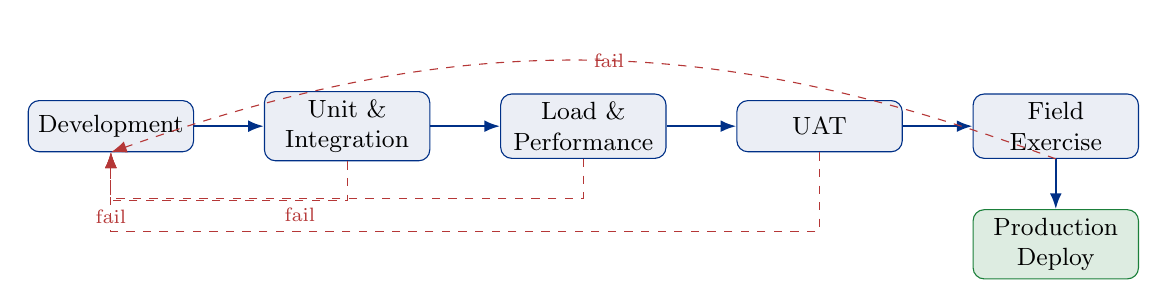
\begin{tikzpicture}[
  font=\small, every node/.style={align=center},
  gate/.style={rounded corners,draw=udblue,fill=udblue!8,
               minimum width=2.1cm,minimum height=0.65cm,inner sep=3pt},
  arr/.style={-{Latex[length=2mm]},thick,udblue},
  fail/.style={-{Latex[length=2mm]},dashed,crit}
]
\node[gate] (g0) at (0,0)    {Development};
\node[gate] (g1) at (3.0,0)  {Unit \&\\Integration};
\node[gate] (g2) at (6.0,0)  {Load \&\\Performance};
\node[gate] (g3) at (9.0,0)  {UAT};
\node[gate] (g4) at (12.0,0) {Field\\Exercise};
\node[gate,fill=low!15,draw=low] (g5) at (12.0,-1.5) {Production\\Deploy};

\draw[arr] (g0) -- (g1);
\draw[arr] (g1) -- (g2);
\draw[arr] (g2) -- (g3);
\draw[arr] (g3) -- (g4);
\draw[arr] (g4) -- (g5);

\draw[fail] (g1.south) -- ++(0,-0.5) -| (g0.south)
  node[midway,below,font=\scriptsize,crit]{fail};
\draw[fail] (g2.south) -- ++(0,-0.5) -| (g0.south)
  node[pos=0.3,below,font=\scriptsize,crit]{fail};
\draw[fail] (g3.south) -- ++(0,-1.0) -| (g0.south);
\draw[fail] (g4.south) to[bend right=20] node[right,font=\scriptsize,crit]{fail} (g0.south);
\end{tikzpicture}
\caption{Quality gate sequence. Each gate must pass before the
next begins. A failure at any gate returns to development.
The field exercise (Level~4) is the only gate that validates
the complete socio-technical system. Source: own elaboration (2026).}
\label{fig:qagate}
\end{figure}

%==========================================================================
\section{Risk Management}
\label{sec:risk}

\subsection{Risk identification methodology.}
We built the risk register in three passes. The first pass took the
five sensitivity parameters identified in our Workshop~1 causal loop
analysis and asked: \emph{what could prevent each mitigation from
working?} The second pass reviewed the three unvalidated
assumptions from Workshop~2 (Table~10 in the revised W2 submission)
and asked: \emph{what happens if each assumption turns out to be
false?} The third pass examined the organisational layer: what
behaviours by campus security staff, students, or university
administration could undermine the system even if the software
works perfectly?

This methodology produced a register that covers technical,
operational, security, \emph{and} behavioural risks. The first
submission covered the first three categories adequately; the
behavioural risks were the gap.

\subsection{Risk register.}
Table~\ref{tab:risks} presents the revised register. Each risk
includes a reference to the Workshop~1 or Workshop~2 finding that
first surfaced it, which is the traceability link between analysis
and risk management that was missing from the previous version.

Risks are scored on a $3\times3$ probability-impact scale.
Probability levels: Low ($<$30\%), Medium (30--60\%), High ($>$60\%).
Impact levels: Low (minor delays), Medium (KPI misses), High
(system objectives unachievable), Critical (safety failure or
legal liability).

{\footnotesize
\begin{longtable}{p{0.5cm}p{4.2cm}p{2.8cm}p{0.9cm}p{0.9cm}p{3.5cm}p{2.5cm}}
\caption{CSAS Risk Register --- Workshop No.\ 3 (Revised)}\label{tab:risks}\\
\toprule
\textbf{ID} & \textbf{Risk (category)} & \textbf{W1/W2 source} & \textbf{Prob.} & \textbf{Imp.} & \textbf{Mitigation} & \textbf{Contingency} \\
\midrule
\endfirsthead
\multicolumn{7}{c}{\small\textit{(continued from previous page)}}\\
\toprule
\textbf{ID} & \textbf{Risk (category)} & \textbf{W1/W2 source} & \textbf{Prob.} & \textbf{Imp.} & \textbf{Mitigation} & \textbf{Contingency} \\
\midrule
\endhead
\bottomrule
\endlastfoot

R-01 & Verification Engine saturates during report surge, exceeds NFR-01 \textit{(Technical)} & W1: non-linear adoption--volume relationship & High & High & Auto-scaling HPA on CPU + queue depth; CRITICAL/SOS bypass path & Manual scale-out; shed STANDARD queue; guard dashboard entry \\[4pt]

R-02 & Push delivery fails; users miss CRITICAL alerts \textit{(Technical)} & W1 benchmarking: platforms fragile on push & Medium & High & Firebase FCM + SMS dual-channel; 10\,s failover timeout & Force SMS; replay from dead-letter queue \\[4pt]

R-03 & GPS degrades on rainy nights; routing misclassifies zones \textit{(Environmental)} & W1: both suspicious events on rainy nights & High & Med. & 20\,m zone buffer; weather API elevates $W_t$ & Manual zone assignment in dashboard \\[4pt]

R-04 & Adoption floor (20--25\%) not reached; crowd verification fails \textit{(Behavioural)} & W1: channel adoption $\approx$12\%; Assumption A1 unvalidated & Med. & High & $\leq$3 interactions; anonymous option; endorsement campaign & Staff-only moderation; delays Phase~2 exit \\[4pt]

R-05 & Security staff do not adopt CSAS dashboard workflow \textit{(Organisational)} & W1 interviews: no existing centralised tool; change resistance likely & Med. & Crit. & Staff training; workflow protocol (Sec.~\ref{sec:implementation}); on-call schedule & Escalation to management; mandatory use policy \\[4pt]

R-06 & Personal data breach (location, incidents) \textit{(Security)} & W2: three personal data categories under Ley~1581 & Low & Crit. & TLS~1.3; AES-256 at rest; RBAC; audit log; pen testing & Isolate service; rotate credentials; notify authority within 72\,h \\[4pt]

R-07 & False reports trigger alert fatigue (Loop~B1) \textit{(Behavioural)} & W1 CLD: Balancing Loop B1 explicitly identified & High & Med. & AI plausibility scorer (DDR-01); user reputation; anon.\ rate limit (3/h) & Human review queue; alert threshold elevation \\[4pt]

R-08 & University does not approve data-processing agreement \textit{(Organisational)} & W2 Assumption A5: institutional integration only partially supported & Med. & High & Sprint~1 engagement; legal review; SIURE as precedent & Design valid; deployment postponed \\[4pt]

R-09 & SMS provider outage; no fallback channel \textit{(Technical)} & W2: Twilio single-provider dependency & Low & High & Active-active two-provider SMS; USSD fallback & Push-only mode; in-app notification \\[4pt]

R-10 & Connectivity dead zones block report submission \textit{(Environmental)} & W2 Assumption A3: signal coverage unvalidated & Med. & Med. & Offline queue + retry; SMS fallback; Sprint~1 connectivity audit & Delayed reporting accepted; mark zones as offline-risk \\[4pt]

R-11 & AI scorer degrades silently over time (model drift) \textit{(Technical)} & W2 DDR-01: model drift is a stated failure condition & Low & High & Monthly retraining; human-override-rate as proxy metric & Disable AI; human-only moderation until retraining \\[4pt]

R-12 & Privacy concerns reduce reporting willingness \textit{(Behavioural)} & W1: harassment incidents require anonymity & Med. & Med. & Anonymous option; location truncated to zone level; public privacy policy & Location-free reporting for sensitive incident types \\[4pt]
\end{longtable}
}% end footnotesize

\subsection{Risk heat map.}
Fig.~\ref{fig:heatmap} positions all twelve risks on the
probability-impact plane. The heat map reveals a cluster of
behavioural and organisational risks in the medium-high region
(R-04, R-05, R-07, R-08) that were largely absent from the
first submission. These risks are not the most dramatic, but
they are the ones most likely to prevent the system from
achieving its stated goals even if the software works correctly.

\begin{figure}[h]
\centering
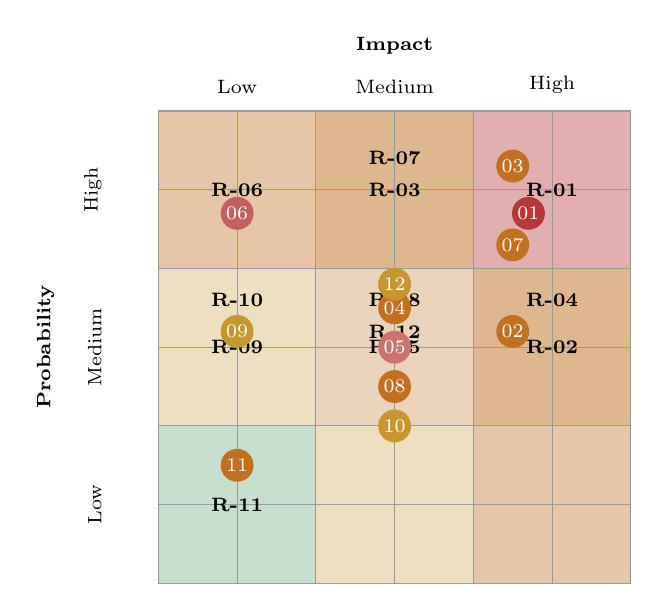
\begin{tikzpicture}[font=\small]
\fill[low!25]  (0,0) rectangle (2,2);
\fill[med!30]  (2,0) rectangle (4,2);
\fill[med!30]  (0,2) rectangle (2,4);
\fill[high!30] (2,2) rectangle (4,4);
\fill[high!40] (4,0) rectangle (6,2);
\fill[high!40] (0,4) rectangle (2,6);
\fill[high!50] (4,2) rectangle (6,4);
\fill[high!50] (2,4) rectangle (4,6);
\fill[crit!40] (4,4) rectangle (6,6);

\draw[black!40] (0,0) grid (6,6);
\node[anchor=south] at (1,6.1) {\scriptsize Low};
\node[anchor=south] at (3,6.1) {\scriptsize Medium};
\node[anchor=south] at (5,6.1) {\scriptsize High};
\node[rotate=90,anchor=south] at (-0.6,1) {\scriptsize Low};
\node[rotate=90,anchor=south] at (-0.6,3) {\scriptsize Medium};
\node[rotate=90,anchor=south] at (-0.6,5) {\scriptsize High};
\node[anchor=south,font=\scriptsize\bfseries] at (3,6.6) {Impact};
\node[rotate=90,anchor=south,font=\scriptsize\bfseries] at (-1.2,3) {Probability};

% Risk positions
\node[font=\scriptsize\bfseries] at (5,5) {R-01};
\node[font=\scriptsize\bfseries] at (5,3) {R-02};
\node[font=\scriptsize\bfseries] at (3,5) {R-03};
\node[font=\scriptsize\bfseries] at (5,3.6) {R-04};
\node[font=\scriptsize\bfseries] at (3,3) {R-05};
\node[font=\scriptsize\bfseries] at (1,5) {R-06};
\node[font=\scriptsize\bfseries] at (5,3) {};
\node[font=\scriptsize\bfseries] at (3,5.4) {R-07};
\node[font=\scriptsize\bfseries] at (3,3.6) {R-08};
\node[font=\scriptsize\bfseries] at (1,3) {R-09};
\node[font=\scriptsize\bfseries] at (3,3) {};
\node[font=\scriptsize\bfseries] at (1,3.6) {R-10};
\node[font=\scriptsize\bfseries] at (1,1) {R-11};
\node[font=\scriptsize\bfseries] at (3,3.2) {R-12};

% Reposition to avoid overlap
\node[circle,fill=crit,inner sep=1pt,font=\scriptsize\color{white}] at (4.7,4.7) {01};
\node[circle,fill=high,inner sep=1pt,font=\scriptsize\color{white}]  at (4.5,3.2) {02};
\node[circle,fill=high,inner sep=1pt,font=\scriptsize\color{white}]  at (4.5,5.3) {03};
\node[circle,fill=high,inner sep=1pt,font=\scriptsize\color{white}]  at (3.0,3.5) {04};
\node[circle,fill=crit!70,inner sep=1pt,font=\scriptsize\color{white}] at (3.0,3.0) {05};
\node[circle,fill=crit!80,inner sep=1pt,font=\scriptsize\color{white}] at (1.0,4.7) {06};
\node[circle,fill=high,inner sep=1pt,font=\scriptsize\color{white}]  at (4.5,4.3) {07};
\node[circle,fill=high,inner sep=1pt,font=\scriptsize\color{white}]  at (3.0,2.5) {08};
\node[circle,fill=med,inner sep=1pt,font=\scriptsize\color{white}]   at (1.0,3.2) {09};
\node[circle,fill=med,inner sep=1pt,font=\scriptsize\color{white}]   at (3.0,2.0) {10};
\node[circle,fill=high,inner sep=1pt,font=\scriptsize\color{white}]  at (1.0,1.5) {11};
\node[circle,fill=med,inner sep=1pt,font=\scriptsize\color{white}]   at (3.0,3.8) {12};
\end{tikzpicture}
\caption{Risk probability-impact heat map. Organisational and
behavioural risks (R-04, R-05, R-08, R-12) appear in the
medium-probability/medium-to-high-impact region --- the zone
that was underrepresented in the first submission.
Source: own elaboration (2026).}
\label{fig:heatmap}
\end{figure}

\subsection{Risk-sprint assignment.}
Risks are not only identified and mitigated in the abstract; they
are assigned to specific sprint activities so that mitigation work
is actually planned and tracked. Table~\ref{tab:risksprinttrace}
maps each high-priority risk to the sprint in which its mitigation
is primarily executed.

\begin{table}[h]
\caption{Risk-to-sprint assignment for high-priority risks}
\label{tab:risksprinttrace}
\centering
\begin{tabularx}{\textwidth}{lXl}
\toprule
\textbf{Risk} & \textbf{Mitigation activity} & \textbf{Sprint} \\
\midrule
R-01 (overload) & Configure and validate Kubernetes HPA; test priority lanes & Sprint~2 \\
R-03 (GPS/weather) & Implement zone-boundary buffer; integrate weather API & Sprint~2 \\
R-04 (adoption floor) & Design and launch institutional endorsement campaign; anonymous option & Sprint~3 \\
R-05 (staff workflow) & Conduct staff training; deploy dashboard; define on-call rotation & Sprint~3 \\
R-06 (data breach) & TLS~1.3 hardening; RBAC implementation; penetration test & Sprint~1--2 \\
R-07 (false reports) & AI scorer integration; user reputation model; anonymous rate limit & Sprint~2 \\
R-08 (legal agreement) & Begin data-processing agreement negotiation with university legal & Sprint~1 \\
R-10 (dead zones) & Conduct campus connectivity audit; configure offline queue & Sprint~1 \\
\bottomrule
\end{tabularx}
\end{table}

%==========================================================================
\section{Project Management Plan}
\label{sec:pm}

\subsection{Why we adopted a hybrid agile approach.}
The first submission used a sequential 12-day Gantt chart and
described it as agile. This was a contradiction that the professor
correctly identified. A Gantt chart with sequential phases
(Planning → Design → Analysis → Integration → Delivery) is a
waterfall schedule, not an agile one.

For this revision, we adopted a \emph{hybrid} approach that is both
honest and appropriate for our context. The outer frame is staged:
four two-week sprints leading to a pilot deployment, followed by
two additional sprints for controlled rollout. Within each sprint,
work follows agile iteration: a sprint goal tied to a system-level
outcome, a backlog of user stories, daily coordination, and a
retrospective. The hybrid is justified because: (i)~a university
project has fixed external deadlines (submission dates) that require
milestone planning; (ii)~some infrastructure work (connectivity
audit, legal agreement) has dependencies that cannot be iteratively
negotiated; but (iii)~the core development work benefits from
short cycles and early user feedback.

\subsection{Product backlog.}
Table~\ref{tab:backlog} presents the product backlog organised by
epic. User stories are written from the perspective of a specific
role (community member, security guard, or security supervisor) so
that their connection to stakeholder needs is visible. Priority is
set by the Workshop~2 requirements traceability matrix: stories
that address the highest-priority functional requirements (FR-01,
FR-02, FR-08) appear in Sprint~1.

\begin{longtable}{p{0.5cm}p{1.0cm}p{5.0cm}p{3.5cm}p{2.0cm}p{1.5cm}}
\caption{Product Backlog}\label{tab:backlog}\\
\toprule
\textbf{ID} & \textbf{Epic} & \textbf{User story} & \textbf{Acceptance criterion} & \textbf{Req.\ trace} & \textbf{Sprint} \\
\midrule
\endfirsthead
\multicolumn{6}{c}{\small\textit{(continued)}}\\
\toprule
\textbf{ID} & \textbf{Epic} & \textbf{User story} & \textbf{Acceptance criterion} & \textbf{Req.\ trace} & \textbf{Sprint} \\
\midrule
\endhead
\bottomrule
\endlastfoot
US-01 & Report & As a community member, I want to submit an incident in $\leq$3 taps so that the friction of reporting doesn't stop me from doing it. & Report submitted with GPS, type, and optional description in under 90\,s in UAT & FR-01, NFR-06 & 1 \\
US-02 & Alert & As a community member near an incident, I want to receive a push alert within 30\,s so that I can take precautions in time. & End-to-end latency $<$30\,s in load test at P95 & FR-02, NFR-01 & 1 \\
US-03 & Emergency & As a student in danger, I want to activate an SOS with one tap so that help is dispatched before I can type anything. & SOS triggers guard notification in $<$4\,s; 90-s escalation path fires if no ACK & FR-08 & 1 \\
US-04 & Verification & As a security guard, I want to see incoming reports ranked by priority so that I can act on the most urgent first. & Dashboard shows CRITICAL alerts at top; guard can approve/reject in $\leq$2 taps & FR-04, NFR-08 & 1 \\
US-05 & Verification & As a community member, I want to confirm or flag a report I can see nearby so that the system uses our collective judgement. & Confirmation increments the verification counter visible to guard & FR-05 & 2 \\
US-06 & Infrastructure & As a system administrator, I want the platform to scale automatically during surges so that alert latency doesn't spike after campus events. & 300\% surge load test passes with 0 CRITICAL alerts exceeding 30\,s & NFR-05 & 2 \\
US-07 & Analytics & As a security supervisor, I want to see a heatmap of this week's incidents so that I can brief the rector without manually compiling reports. & Weekly heatmap generated automatically and accessible from the dashboard & FR-09 & 2 \\
US-08 & Privacy & As a user who reported harassment, I want my identity protected so that I don't face retaliation for reporting. & Reporter identity encrypted at rest; not visible in guard dashboard without supervisor override & FR-01, NFR-04 & 2 \\
US-09 & Adoption & As the security supervisor, I want on-duty guards to receive training before the pilot so that they actually use the dashboard. & 100\% of on-duty guards complete 30-min onboarding session before pilot launch & Org.\ robustness & 3 \\
US-10 & Adoption & As a student, I want to understand the app in under 2 minutes so that I don't have to read a manual. & UAT: 85\% of participants complete onboarding unaided in $<$2 min & NFR-06 & 3 \\
US-11 & Integration & As a security supervisor, I want CSAS to forward verified incidents to SIURE UD automatically so that the official record is complete. & SIURE integration live; verified incident appears in SIURE within 60\,s & FR-07, integration & 3 \\
US-12 & Field exercise & As the project team, we want to validate the complete system under real campus conditions before the pilot so that we know it works outside the lab. & Field drill: $\geq$3 of 4 scenarios pass the end-to-end latency and delivery criteria & System validation & 3 \\
US-13 & Pilot & As the security team, we want to monitor the pilot's KPIs in real time so that we can decide when to proceed to full rollout. & Pilot dashboard shows all 10 KPIs from Table~\ref{tab:accept} in real time & Sprint~4 goal & 4 \\
US-14 & Continuous improvement & As the implementation lead, I want a monthly KPI review process so that degradation is caught before it becomes a crisis. & Monthly review meeting scheduled; corrective-action ticket generated for any sustained KPI miss & Post-pilot & 4 \\
\end{longtable}

\subsection{Sprint plan.}
Table~\ref{tab:sprints} defines the four sprints, each with a
system-level goal (not a list of tasks) and explicit exit criteria.
Exit criteria must be satisfied before the next sprint begins;
unmet criteria are carried forward and may delay the sprint
boundary.

\begin{table}[h]
\caption{Sprint plan with system-level goals and exit criteria}
\label{tab:sprints}
\centering
\begin{tabularx}{\textwidth}{p{1.4cm}Xp{4.0cm}p{3.5cm}}
\toprule
\textbf{Sprint} & \textbf{System-level goal} & \textbf{User stories} & \textbf{Exit criteria} \\
\midrule
Sprint~1 (weeks 1--2) & \textbf{Core reporting and alerting chain is operational.} A community member can submit a report and a security guard can receive a CRITICAL alert on a staging environment within the NFR-01 target. & US-01, US-02, US-03, US-04 & All four stories pass UAT; end-to-end latency $<$30\,s on staging; campus connectivity audit complete; R-08 engagement initiated \\[6pt]
Sprint~2 (weeks 3--4) & \textbf{The system is robust and verifiable.} Crowd verification, auto-scaling, analytics, and privacy protections are in place and validated under simulated load. & US-05, US-06, US-07, US-08 & 300\% surge test passes; false-positive rate $<$5\% in staging; heatmap renders correctly; anonymous reporter encryption verified \\[6pt]
Sprint~3 (weeks 5--6) & \textbf{The socio-technical system is ready for real users.} Security staff are trained, the SIURE integration is live, and a field exercise confirms the complete system works on campus. & US-09, US-10, US-11, US-12 & 100\% guard onboarding complete; field exercise $\geq$3/4 scenarios pass; SIURE integration confirmed; data-processing agreement signed \\[6pt]
Sprint~4 (weeks 7--8) & \textbf{The pilot is running and improving.} The system is in live use with the pilot cohort, KPIs are being measured, and the first retrospective has produced actionable improvements. & US-13, US-14 & Adoption $\geq$20\% of pilot cohort; guard acknowledgement rate $\geq$90\% on CRITICAL alerts; first retrospective held; no open critical risks \\[6pt]
\bottomrule
\end{tabularx}
\end{table}

\subsection{Team roles and responsibilities.}
The four-member team maps to four specialised roles.
Table~\ref{tab:roles} specifies the primary responsibility of each
role and the sprint deliverables they own. Roles are assigned
to align technical strengths with the demands of each sprint phase.

\begin{table}[h]
\caption{Team roles, responsibilities, and sprint ownership}
\label{tab:roles}
\centering
\begin{tabularx}{\textwidth}{lXX}
\toprule
\textbf{Role} & \textbf{Responsibilities} & \textbf{Sprint ownership} \\
\midrule
Project Manager (Persona~1) & Sprint planning, coordination, blocker escalation, stakeholder communication; owns the sprint review and retrospective process & All sprints: daily coordination, weekly progress report, sprint review facilitation \\
Architecture \& Quality Lead (Persona~2) & System and software architecture; quality framework; standards alignment; TLS/security configuration & Sprint~1--2: core architecture; quality gate setup; load test design \\
Risk \& Integration Lead (Persona~3) & Risk register maintenance; SIURE integration; third-party APIs; legal agreement coordination; data protection compliance & Sprint~1--3: connectivity audit; R-08 engagement; SIURE bridge; penetration test \\
Implementation \& Evolution Lead (Persona~4 --- Felipe Garzón) & Executive summary; ethics; implementation strategy; field exercise coordination; GitHub management; conclusions; W1→W3 evolution narrative & Sprint~3--4: field exercise; pilot dashboard; monthly KPI review process; repository \\
\bottomrule
\end{tabularx}
\end{table}

\subsection{Sprint ceremonies and communication.}
Each sprint includes four standard ceremonies:
(i)~\textbf{Sprint planning} (2\,h at sprint start): review backlog,
commit to sprint goal, assign stories to members;
(ii)~\textbf{Daily stand-up} (15\,min asynchronous via WhatsApp):
progress, blockers, dependencies;
(iii)~\textbf{Sprint review} (1\,h at sprint end): demo working
software or completed artefact to at least one representative
user (a classmate or the instructor);
(iv)~\textbf{Sprint retrospective} (45\,min at sprint end): what
worked, what did not, one concrete improvement for next sprint.

Any blocker unresolved for more than 24 hours is escalated to the
Project Manager. Any blocker that cannot be resolved within the
sprint is escalated to the course instructor with a written impact
assessment.

%==========================================================================
\section{Implementation Strategy}
\label{sec:implementation}

\subsection{Overview.}
The implementation strategy describes how the system --- the
complete socio-technical system, not just the software --- moves
from design to live operation. The three-phase deployment
inherited from Workshop~2 (Pilot → Controlled rollout → Full
operation) remains valid; this section adds the organisational
change management layer that was absent from the first submission.

\subsection{Organisational change management.}
The most underspecified aspect of the first submission was what
happens on the human side before the pilot launches. Our Workshop~1
interviews made clear that the current campus security workflow
relies on phone calls and walk-up reports; adopting a
dashboard-mediated workflow requires intentional change management,
not just software deployment.

Three activities must be completed before the Phase~1 pilot begins
and are tracked as US-09 in the sprint backlog:

\begin{enumerate}
\item \textbf{Workflow protocol definition.} In collaboration with the
  security supervisor, we define the new operational procedure:
  which alerts require guard acknowledgement within what time,
  how the dashboard replaces the current paper log, and how
  escalation to local authorities is handled through the system
  rather than by phone. This protocol is documented and
  approved before training begins.

\item \textbf{Security staff training programme.} All on-duty guards
  attend a 30-minute session that covers: how to access the
  dashboard, how to interpret priority tiers, how to approve
  or reject a report, and how to activate the authority
  escalation path. The session is followed by a 15-minute
  supervised exercise using a test account. Completion is
  logged and is a hard prerequisite for the field exercise.

\item \textbf{Student and faculty communication campaign.}
  The system is announced through official university channels
  (email, physical posters in high-traffic areas, a 2-minute
  video on the university's internal platform). The campaign
  emphasises anonymity, simplicity, and the concrete
  improvement in safety it enables. The goal is to reach the
  20--25\% adoption floor within the four-week pilot.
\end{enumerate}

\subsection{Phase 1 --- Pilot (4 weeks, Sprint~4).}
The pilot is restricted to a single faculty building and a closed
cohort of approximately 200 registered users (students, faculty,
and two on-duty guards). All reports during the pilot are
monitored in real time by the Architecture Lead and Risk Manager.
Exit criteria: all KPIs in Table~\ref{tab:accept} met for two
consecutive weeks; adoption floor ($\geq$20\%) reached; zero open
critical risks; guard acknowledgement rate $\geq$90\% on CRITICAL
alerts.

\subsection{Phase 2 --- Controlled rollout (8 weeks).}
The system is extended to the full campus using feature flags that
control which user cohorts have access to which features. The
campus-wide connectivity audit completed in Sprint~1 informs which
zones require enhanced SMS fallback configuration. Exit criteria:
adoption $\geq$30\% of total target population; delivery success
$\geq$99.5\% in real conditions; no open high-severity risks.

\subsection{Phase 3 --- Full operation (continuous).}
The system is declared production-grade. Monthly KPI reviews,
quarterly risk reassessments, and annual architecture reviews
(ISO~9001 management review) govern its continuous improvement.

\subsection{Infrastructure readiness checklist.}
The system is cleared for Phase~1 deployment when the following
indicators are simultaneously satisfied: (i)~architecture sign-off
by Architecture Lead; (ii)~campus connectivity audit complete;
(iii)~no open critical risks; (iv)~Level~4 field exercise passed;
(v)~TLS/security scan clean; (vi)~data-processing agreement signed;
(vii)~all on-duty guards trained; (viii)~on-call rotation defined
and documented.

%==========================================================================
\section{Evolution from Workshops 1--3}

\subsection{Requirements traceability.}
Table~\ref{tab:reqtrace} closes the traceability loop from Workshop~1
empirical findings through Workshop~2 requirements to the Workshop~3
robustness and project decisions. This table was missing from the
first submission; it is the most direct demonstration that the design
emerges from the system analysis rather than from generic software
engineering practice.

\begin{table}[h]
\caption{End-to-end requirements traceability: W1 finding → W2 requirement → W3 decision}
\label{tab:reqtrace}
\centering
\begin{tabularx}{\textwidth}{p{3.5cm}p{3.2cm}p{4.0cm}p{3.5cm}}
\toprule
\textbf{W1 empirical finding} & \textbf{W2 requirement / DDR} & \textbf{W3 robustness / quality / risk decision} & \textbf{Sprint that validates it} \\
\midrule
Only 41\% of incidents recorded; high friction in reporting & FR-01: $\leq$3-interaction reporting & US-01; R-04 mitigation (adoption campaign); Level~3 UAT acceptance $\geq$85\% completion & Sprint~1 (story), Sprint~3 (campaign) \\
All suspicious events at night (18:00--22:00), parking lot zone & DDR-02: time weight $W_t=1.5$ for 18:00--22:00; NFR-03: guaranteed availability in window & Technical robustness Table~\ref{tab:techrobust}: multi-AZ guaranteed during this window; R-03 mitigation for GPS degradation & Sprint~2 (infra), Sprint~1 (availability) \\
Low reporting culture; 12\% channel adoption & DDR-01: friction $\to$ hybrid verification; FR-01: anonymous option & Adoption floor requirement (20--25\% before Phase~2); R-04 (behavioural risk); US-09--10 (training and onboarding) & Sprint~3 \\
Staff: no centralised tool; 11.4 min latency & FR-04: security dashboard; FR-08: SOS bypass & R-05 (staff workflow change as critical risk); US-04 (dashboard story); field exercise (Level~4 validation); org.\ robustness Section~2.3 & Sprint~1 (dashboard), Sprint~3 (training) \\
Rainy nights: both suspicious events coincident & W2 operational scenario 1 (rain condition) & R-03 mitigation: weather API, GPS buffer, proactive SMS; environmental robustness Section~2.4 & Sprint~2 \\
GPS signal not assessed on campus & W2 Assumption~A3: connectivity unvalidated & R-10: connectivity dead-zone risk; Sprint~1 prerequisite: connectivity audit before Phase~1 clearance & Sprint~1 \\
\bottomrule
\end{tabularx}
\end{table}

\subsection{Design maturity progression.}
Looking across the three workshops, the most significant maturation
is the shift from implicit to explicit claims. In Workshop~1, risks
were surfaced in the assumptions section but not quantified. In
Workshop~2, mitigation mechanisms were designed but justified only
in Design Decision Records. In Workshop~3, every risk is registered
with a probability, an impact, a mitigation with a sprint assignment,
and a contingency. Every quality attribute has an acceptance criterion
expressed as an observable system outcome. And every project activity
is traceable to a user story that is traceable to a stakeholder need
that is traceable to a Workshop~1 empirical finding.

The lesson we draw from this progression is practical: a design
becomes robust not by adding mechanisms but by making the chain from
evidence to decision to validation explicit enough that someone
external to the team can follow and challenge it.

%==========================================================================
\section{Ethical and Legal Considerations}

The ethical framework established in Workshop~2 is retained in
full; this section adds the considerations that emerged specifically
from the Workshop~3 robustness and risk analysis.

\subsection{Data protection under Ley 1581/2012.}
The system complies with Ley~1581 de 2012 on four binding
obligations: (i)~explicit informed consent at registration,
purpose-bound to campus safety; (ii)~data processed only for
declared safety purposes; (iii)~user rights of access, correction,
and deletion supported by the User Service; (iv)~12-month retention
policy with irreversible anonymisation thereafter. R-06 (data breach)
and R-12 (privacy concerns reducing adoption) are the two risks most
directly linked to this framework and are mitigated accordingly.

\subsection{Algorithmic accountability.}
The AI plausibility scorer (DDR-01) makes automated decisions that
affect whether an incident reaches the security team. This creates
a transparency obligation: the scoring criteria, confidence thresholds,
and human-override rate are logged and reviewed monthly. Any
sustained increase in the human-override rate is treated as a
leading indicator of model drift (R-11) and triggers retraining.

\subsection{Misuse prevention.}
Three misuse vectors are addressed by design: false reporting
(AI scorer + user reputation + anonymous rate limit); harassment
through the platform (immutable audit log); weaponisation against
innocent parties (human-in-the-loop for highest-severity alerts
before authority escalation). We recognise that the last mechanism
introduces a 90-second window of human deliberation that may be
too slow in a genuine life-threatening situation; this is an
explicit design trade-off, not an oversight, and it will be
re-evaluated after the pilot based on observed response patterns.

\subsection{Equity.}
The SMS/USSD fallback and the Spanish-first, low-literacy interface
prevent the system from being inaccessible to campus members without
smartphones or with intermittent connectivity. The adoption campaign
(US-09, US-10) is designed to reach all user groups, not only the
technically proficient.

%==========================================================================
\section{Repository Management}

All Workshop~3 artefacts are stored in the
\texttt{workshop3\_revised/} folder of the GitHub repository at
\texttt{github.com/filipghs/Systems-Analysis}, following the
convention established for Workshops~1 and~2. The folder structure is:

\begin{itemize}
\item \texttt{docs/} --- this PDF and its \LaTeX{} source.
\item \texttt{diagrams/} --- TikZ sources for Figs~\ref{fig:qagate} and~\ref{fig:heatmap}.
\item \texttt{risk\_register/} --- CSV export of Table~\ref{tab:risks} for spreadsheet tooling.
\item \texttt{backlog/} --- CSV export of Table~\ref{tab:backlog} for project management tooling.
\item \texttt{README.md} --- updated navigation index covering all three workshops.
\end{itemize}

The main branch is protected; every change reaches it through a pull
request reviewed by at least one team member other than the author.

%==========================================================================
\section{Conclusions}

Workshop~3 completes the CSAS project cycle by adding the robustness,
quality, risk, and project management layers that were outlined in
Workshop~2 but not yet fully specified. Four conclusions summarise
what this workshop contributed.

\paragraph{Robustness requires three layers.}
Technical hardening alone is insufficient. Our fieldwork showed
that the conditions most likely to cause system failure are
environmental (rainy nights degrade GPS and connectivity) and
organisational (security staff do not change their workflow). Both
layers are now explicitly addressed: environmental robustness through
weather-adaptive routing and proactive SMS fallback; organisational
robustness through the workflow protocol, staff training programme,
and adoption floor requirement.

\paragraph{Risk management must include behavioural risks.}
The risk register in the first submission covered technical,
security, and operational categories. The most consequential gaps
were in the behavioural and organisational categories: adoption
failure (R-04), staff workflow resistance (R-05), and student privacy
concerns reducing willingness to report (R-12). These risks
cannot be mitigated by software mechanisms; they require community
engagement, institutional endorsement, and sustained monitoring of
adoption metrics.

\paragraph{Agile planning is substantively different from waterfall scheduling.}
The sprint plan in this revision replaced a sequential Gantt chart
with a structure in which each sprint has a \emph{system-level goal}
(not a task list), a backlog of user stories traceable to stakeholder
needs, and exit criteria that measure observable system behaviour.
The difference is not cosmetic: the sprint goals force us to define
what ``done'' means in terms of user outcomes rather than activities
completed.

\paragraph{Traceability is the thread that holds the design together.}
The end-to-end traceability table (Table~\ref{tab:reqtrace}) makes
visible what was implicit across the three workshops: every design
decision traces to a specific Workshop~1 empirical finding, and every
Workshop~3 risk or quality criterion traces to a Workshop~2 design
choice. Without this thread, the design could not be audited,
challenged, or improved --- it would simply be a collection of
decisions without a rationale.

%==========================================================================
\section*{References}
\addcontentsline{toc}{section}{References}
\begin{enumerate}[label={[\arabic*]},leftmargin=1.5em,itemsep=2pt]
\item Garzón Herrera, F.~J. et al., \emph{Workshop No.\ 1: Systems Analysis of the CSAS}, Universidad Distrital Francisco José de Caldas, 2026.
\item Garzón Herrera, F.~J. et al., \emph{Workshop No.\ 2: System Design of the CSAS (Revised)}, Universidad Distrital Francisco José de Caldas, 2026.
\item ISO, \emph{ISO 9001:2015 --- Quality Management Systems --- Requirements}, ISO, Geneva, 2015.
\item ISO/IEC, \emph{ISO/IEC 25010:2011 --- SQuaRE --- System and Software Quality Models}, 2011.
\item ISO, \emph{ISO 31000:2018 --- Risk Management --- Guidelines}, ISO, Geneva, 2018.
\item IEEE, \emph{IEEE Std 830-1998 --- Recommended Practice for Software Requirements Specifications}, 1998.
\item IEEE, \emph{IEEE Std 1633-2016 --- Recommended Practice on Software Reliability}, 2016.
\item IEEE/ISO/IEC, \emph{ISO/IEC/IEEE 12207:2017 --- Software Life Cycle Processes}, 2017.
\item CMMI Institute, \emph{CMMI for Development, Version 2.0}, ISACA, 2018.
\item PMI, \emph{PMBOK Guide}, 7th ed., PMI, 2021.
\item Congreso de Colombia, \emph{Ley 1581 de 2012 --- Régimen General de Protección de Datos Personales}, 2012.
\end{enumerate}

\end{document}
